% A字 例1：AD=3, DB=2, BC=10, 求 DE=6
\documentclass[tikz,border=4pt]{standalone}
\usepackage{ctex}
\usepackage{amsmath}
\usetikzlibrary{calc}
\begin{document}
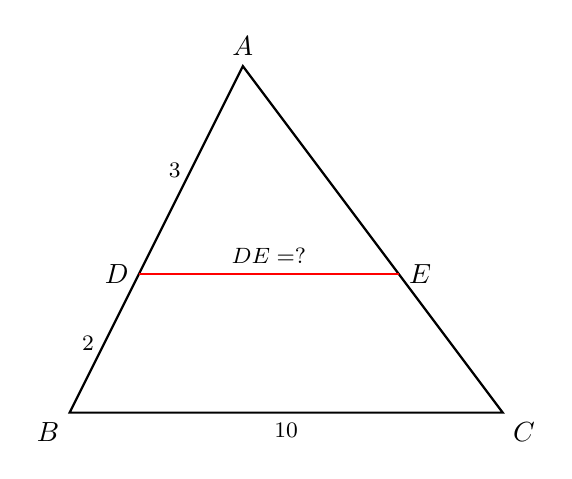
\begin{tikzpicture}[scale=0.55, thick]
  \coordinate (A) at (4,8);
  \coordinate (B) at (0,0);
  \coordinate (C) at (10,0);
  % AD=3, AB=5 so D = A + (3/5)(B-A)
  \coordinate (D) at ($(A)!0.6!(B)$);
  \coordinate (E) at ($(A)!0.6!(C)$);
  \draw (A)--(B)--(C)--cycle;
  \draw[red] (D)--(E);
  \node[above] at (A) {$A$};
  \node[below left] at (B) {$B$};
  \node[below right] at (C) {$C$};
  \node[left] at (D) {$D$};
  \node[right] at (E) {$E$};
  \node[left] at ($(A)!0.3!(B)$) {\footnotesize $3$};
  \node[left] at ($(D)!0.5!(B)$) {\footnotesize $2$};
  \node[below] at ($(B)!0.5!(C)$) {\footnotesize $10$};
  \node[above] at ($(D)!0.5!(E)$) {\footnotesize $DE=?$};
\end{tikzpicture}
\end{document}
